\vspace{-20pt}
\section{Evaluation}\label{sec:evaluation}
\vspace{-15pt}

To evaluate our approach under varying stack conditions and SEU injection rates, three AVR applications are considered. The stack usage pattern of each application is shown in Figure \ref{fig:stacksize_usage}.
\vspace{-15pt}
\subsection{Validation}
\vspace{-20pt}
We first validate our approach and consider the SEU protection efficacy it affords. In our analysis, we ignore both the \texttt{.data} and the \texttt{.bss} sections, as well as the heap section. Data stored in the \texttt{.data}, \texttt{.bss}, and \texttt{heap} sections can be protected using well-known techniques based on cloning and comparison. We focus our analysis on stack frame protection.
\vspace{-20pt}
\begin{figure}
	\centering
	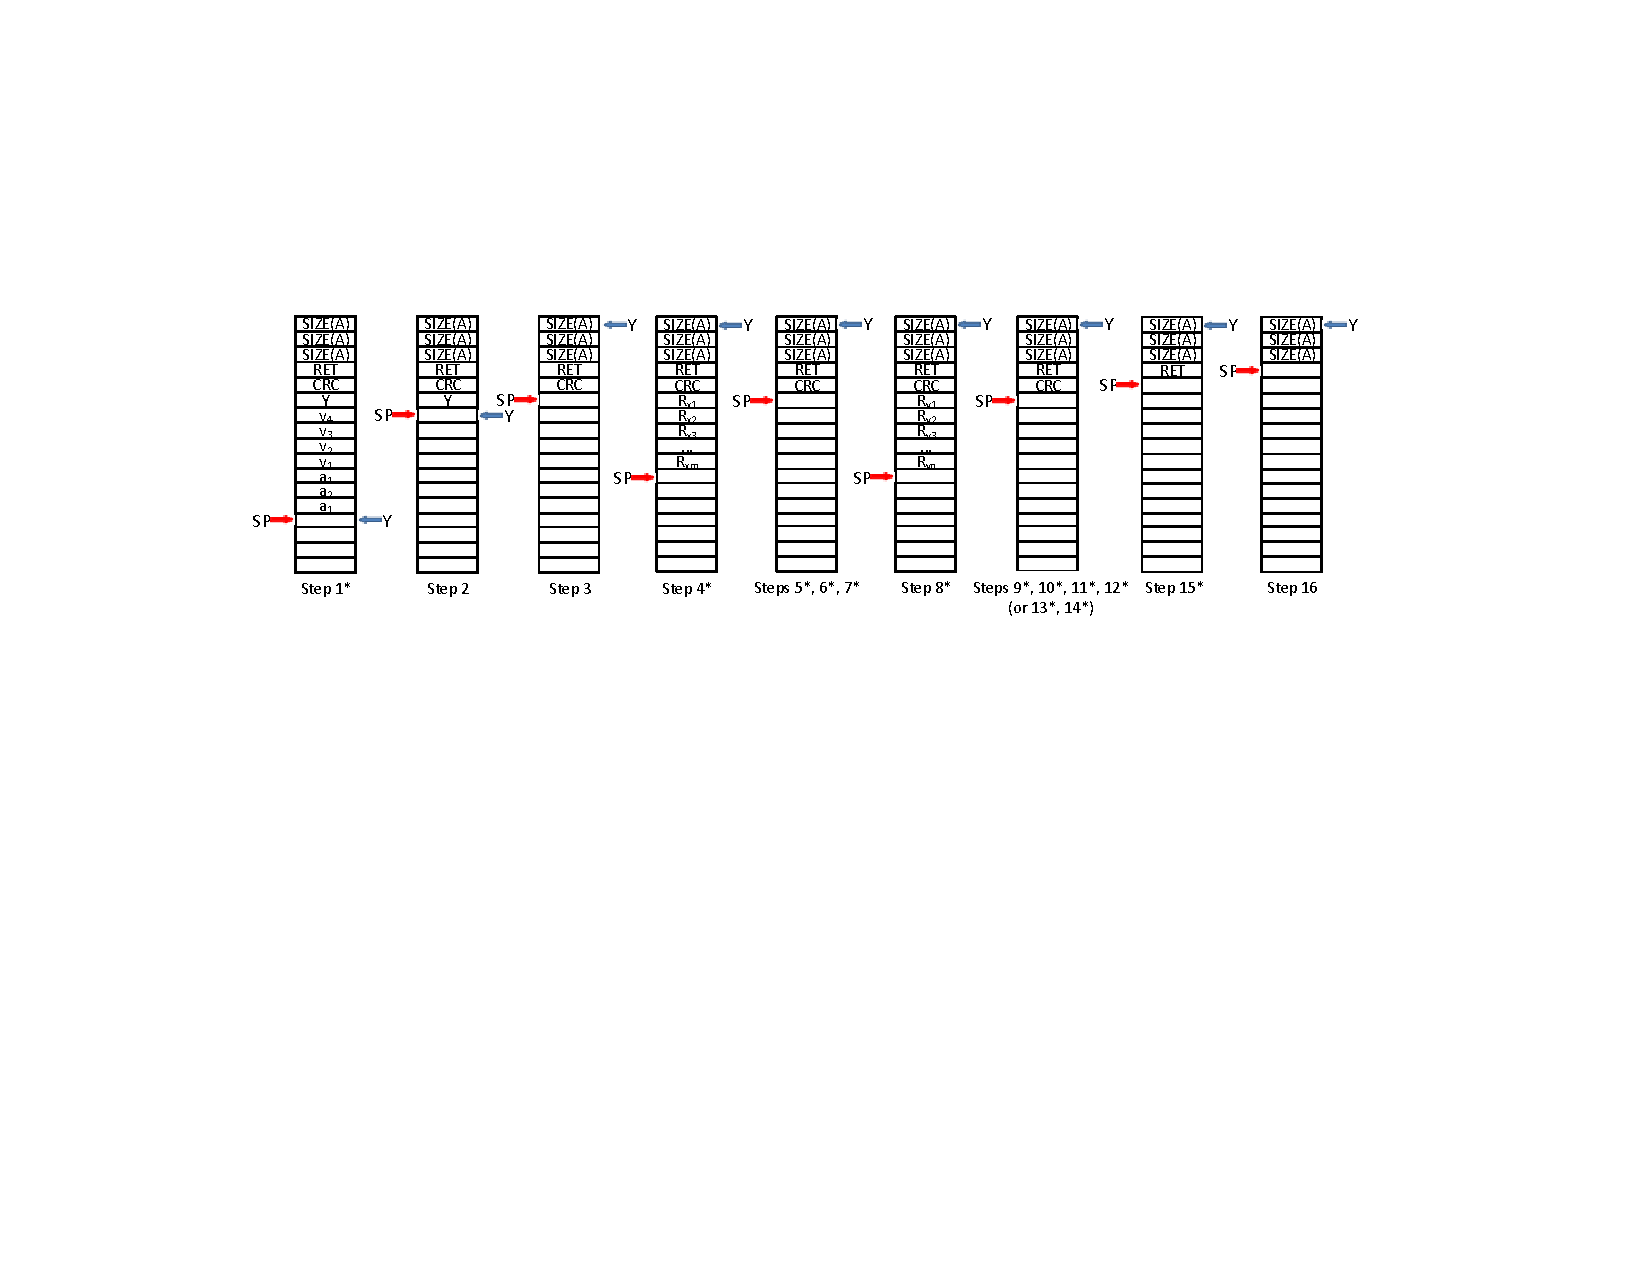
\includegraphics[width=1.0\textwidth]{figures/modified_function_operations_stack_post_execution_v3}
	\vspace{-20pt}
	\caption{Modified Function Return Process}\label{fig:modified_function_operation_post_execution}
\end{figure}
\vspace{-25pt}
We first assume that the currently executing function's frame, which includes the return address of the injected code segment, is not affected by SEUs. The stack frames of callers and callees are guaranteed to be correct, so the stack is guaranteed to be correct. To verify this claim, the AVR Simulator IDE~\cite{avrsimide} was used to manually inject SEUs, and to observe execution results. The results showed that each function is able to detect and fix SEUs introduced ``beneath'' the topmost stack frame.

However, if the stack frame of the current function is affected by an SEU, protection is not guaranteed. If the SEU changes key data, such as the return address or stack frame size, the current function will not execute as expected. 
\begin{wrapfigure}{l}{0.5\textwidth}
	\vspace{-25pt}
	\begin{center}
		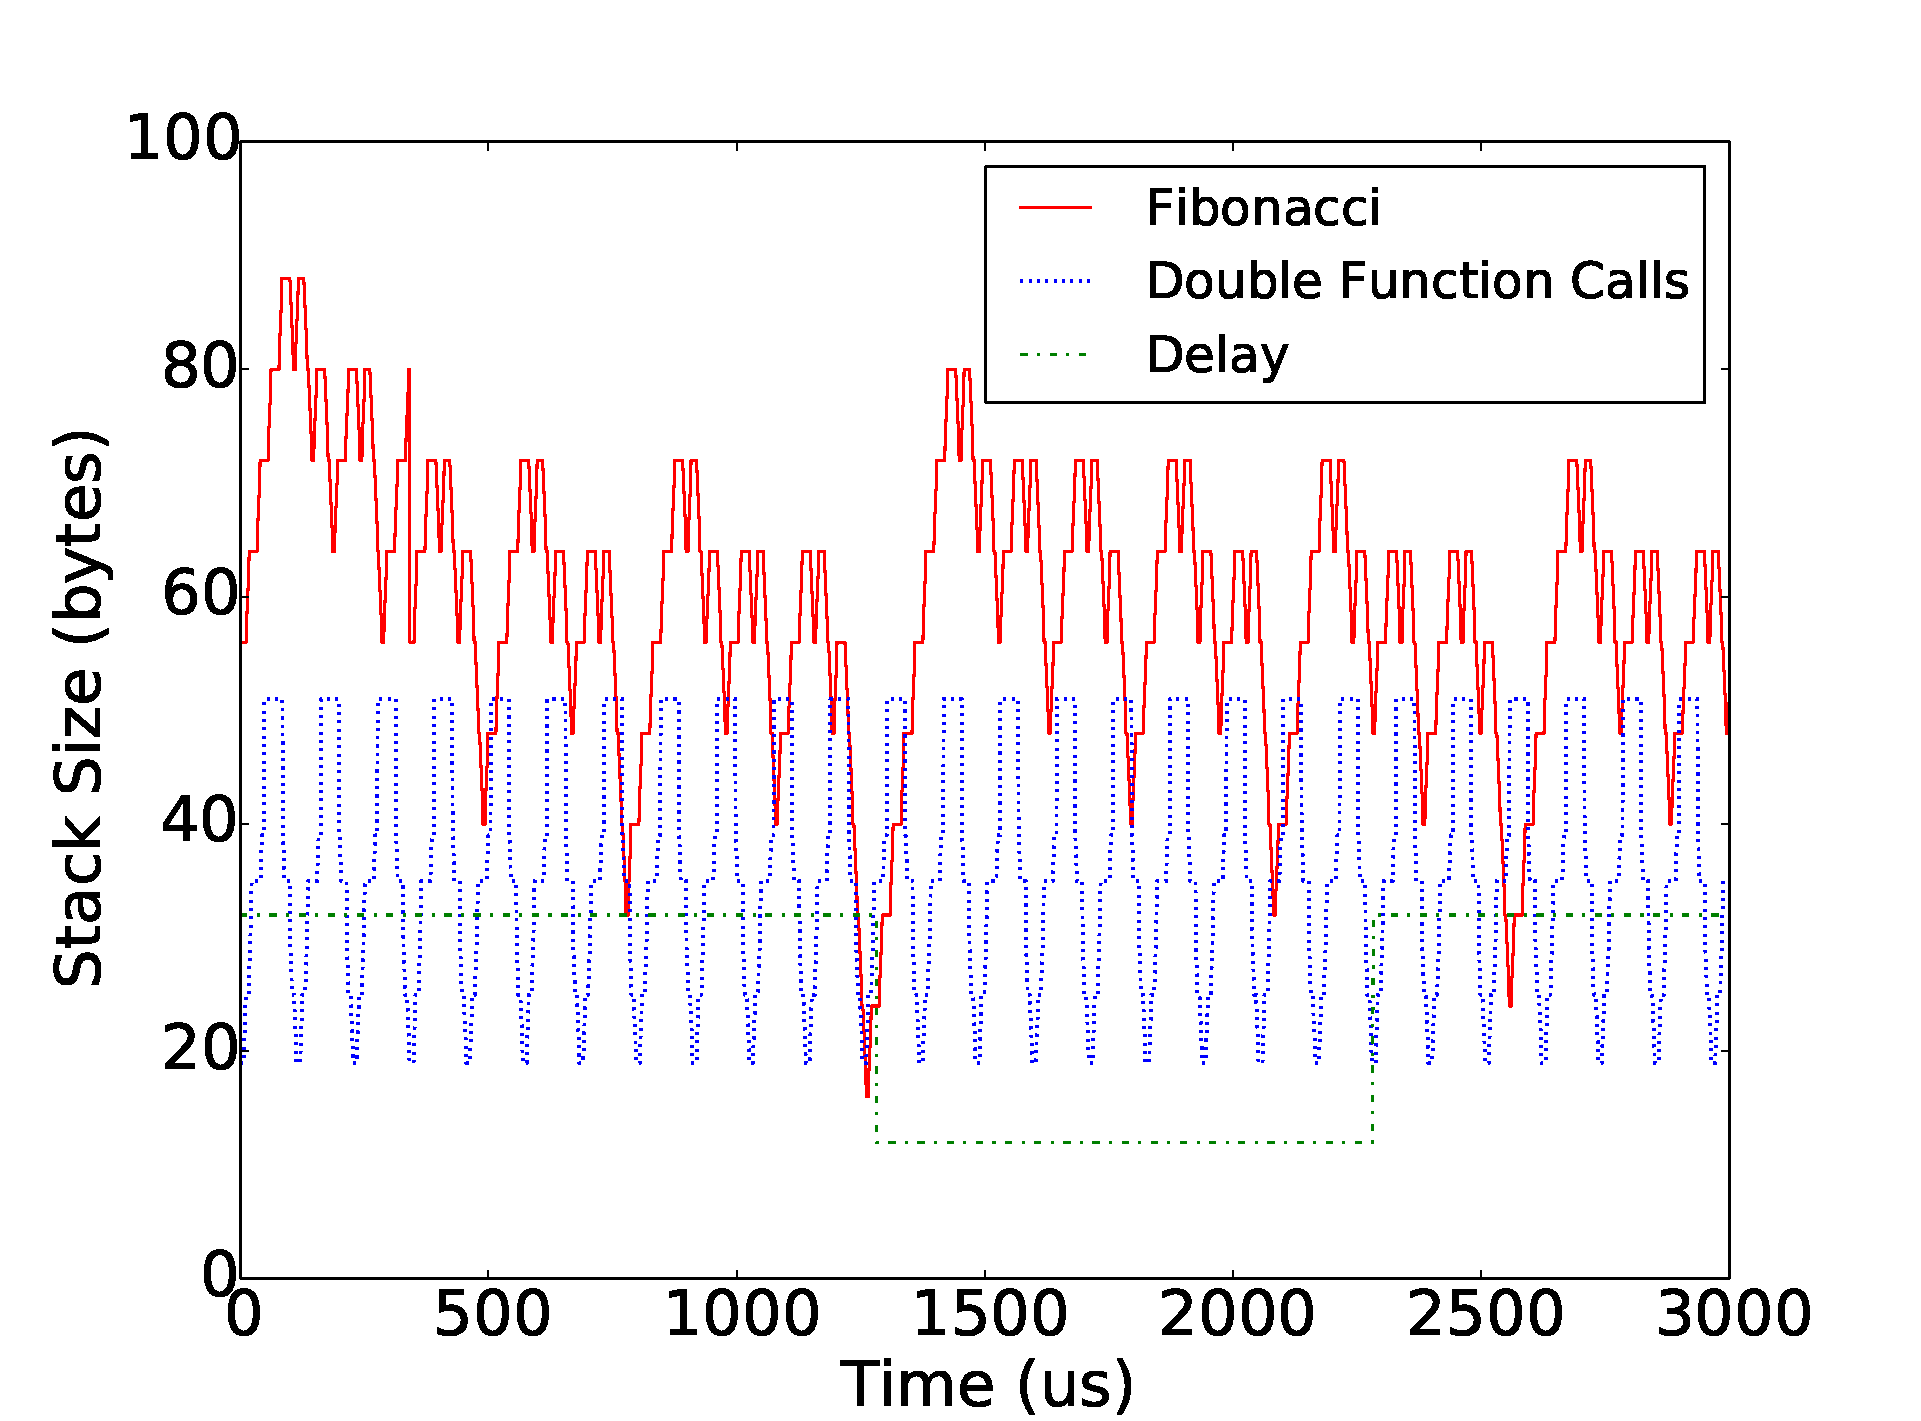
\includegraphics[width=0.5\textwidth]{figures/stacksize_usage_v3.pdf}
	\end{center}
	\vspace{-20pt}
	\caption{Stack Usage of Test Applications}\label{fig:stacksize_usage}
	\vspace{-25pt}
\end{wrapfigure}
We assume that only one SEU will occur during a given function execution, and that the SEU is uniformly likely to affect all bits in RAM. The probability of successful SEU protection can be expressed as $p=1-c/(2s+e-c+6)$. Where $p$ is the probability of successful protection, $s$ is the stack size, $e$ is the size of the unused space in RAM, $6$ is the size of the three STP copies, and $c$ is the average size of a stack frame. Since the return address of the injected code segment is stored in the current stack frame, the two bytes for the return address are included in c. The total size of protected memory is $s+e+(s-c)+6$, where $s-c$ is the size of the stack frame copies stored in the \textit{md} section.

We extend our analysis to cases where more than one SEU may occur during a given function execution. Due to lack of space, we omit the derivation details. The (conservative) probability of successful protection can be expressed as:
\vspace{-5pt}
\begin{equation}\label{eq_seu2}
\scriptsize
\begin{split}
&p=(1-\frac{c}{2s+e-c+6})^n*(1-\frac{6}{2s+e-2c+6})^n \\
&*(1-\frac{6}{2s+e-2c})^n*\{(1-\frac{2c}{2s+e-2c-6})^n \\
&+ \mathrm{C}_2^1*(1-\frac{c}{2s+e-2c-6})^n*[1-(1-\frac{c}{2s+e-3c-6})^n]\}
\end{split}
\end{equation}

Where $p$ is the probability of success, $s$ is the size of the stack, $e$ is the size of the unused space in RAM, $6$ is the size of the three stack frame size copies or the three STP copies, $c$ is the average size of the stack frame (including the return address of the injected code segment), and $n$ is the number of SEUs that occur during a function's execution. In equation \ref{eq_seu2}, the number of SEUs that occur, $n$, can be expressed as $n=y*l*f/m$, where $y$ is the number of clock cycles used to execute each instruction, $m$ is the frequency of the microprocessor, $l$ is the average number of function instructions, and $f$ is the SEU injection rate. Most AVR instructions require 2 clock cycles to execute, and the frequency of our ATmega644 is set to 10MHz.

We now consider the relationship between SEU protection probability and SEU occurrence rate. To demonstrate the relationship, we collect the corresponding parameters for the three test applications using AVR Simulator IDE. Figure \ref{fig:success_probability} plots the change in SEU protection probability as a function of SEU injection rate. The x-axis represents the rate at which SEUs are injected, and the y-axis represents the corresponding SEU protection probability. Each vertical line 
\begin{wrapfigure}{l}{0.5\textwidth}
	\vspace{-25pt}
	\begin{center}
		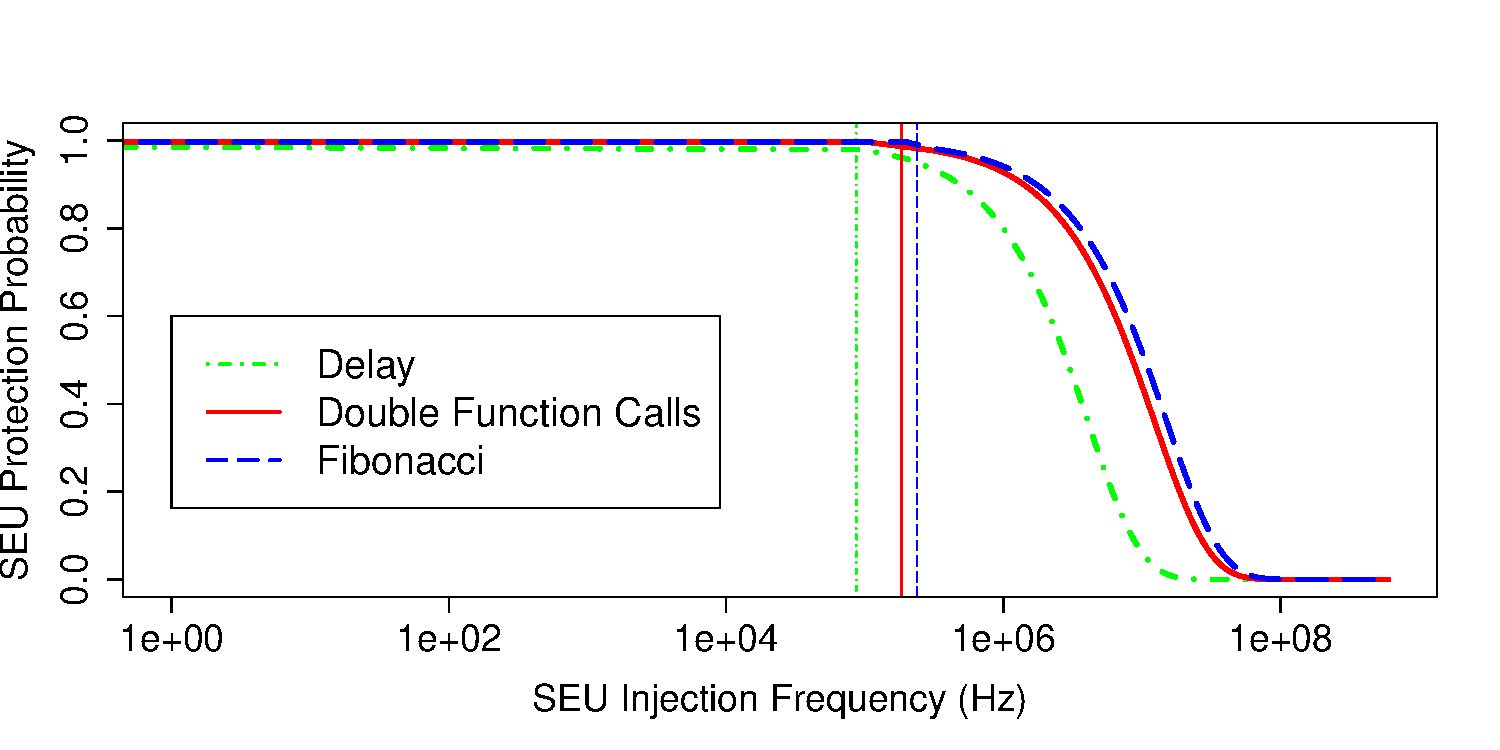
\includegraphics[width=0.5\textwidth, height=80pt]{figures/success_probability_v2.pdf}
	\end{center}
	\vspace{-15pt}
	\caption{SEU Protection Probability}
	\vspace{-25pt}
	\label{fig:success_probability}
\end{wrapfigure}
marks where the number of SEUs begins to exceed 1 (for each application). When only one SEU occurs during a given function execution (left side of the vertical line), the SEU protection probability is constant (Delay: 99.48\%, Double Function Calls: 99.71\%, Fibonacci: 99.68\%) because the only case the approach cannot handle is when the current frame is affected. When more than one SEU occurs during a given function execution (right side of the vertical line), the SEU protection probability increases. As the SEU occurrence rate increases, the SEU protection probability decreases, until it approaches 0. The lower the stack dynamism, the longer the function execution time, which increases the probability of SEU occurrence in the current stack frame.
\vspace{-15pt}
\subsection{Performance}
\vspace{-10pt}
Since the same code is injected for every function, the execution overhead is similar for all functions, varying only when an SEU is detected. The execution overhead depends on the size of the (recovered) stack frame. The \textit{CRC Calculate} code segment and \textit{STP Update} code segment execute twice for each function, and the \textit{Frame Copy} code segment executes either once or twice, depending on whether an SEU is detected. Each of the other code segments executes once for each function execution. The minimum overhead introduced in terms of number of clock cycles is $62*S+304$, when an SEU is not detected. The worst case is $70*S+432$ clock cycles, when an SEU is detected. 

We next evaluate space overhead using the three test applications. The ROM space data was collected using \textit{avr-size}. The results are summarized in Figure \ref{fig:space_overhead}. The y-axis represents ROM size, in bytes. Delay and Fibonacci involve two functions, and Double Function Calls involves four. From Figure \ref{fig:space_overhead}, we can see that the ROM overhead for the Double Function Calls application is twice the Delay and Fibonacci applications. ROM overhead is related only to the number of functions in the program.
\vspace{-15pt}
\subsection{Physical Hardware}
\vspace{-5pt}
To validate our approach on physical hardware, we emulate the occurrence of SEUs by flipping random bits in the target SRAM area. To perform auditable test runs, we developed an AVR application which continuously generates an 
\begin{wrapfigure}{l}{0.3\textwidth}
	\vspace{-30pt}
	\begin{center}
		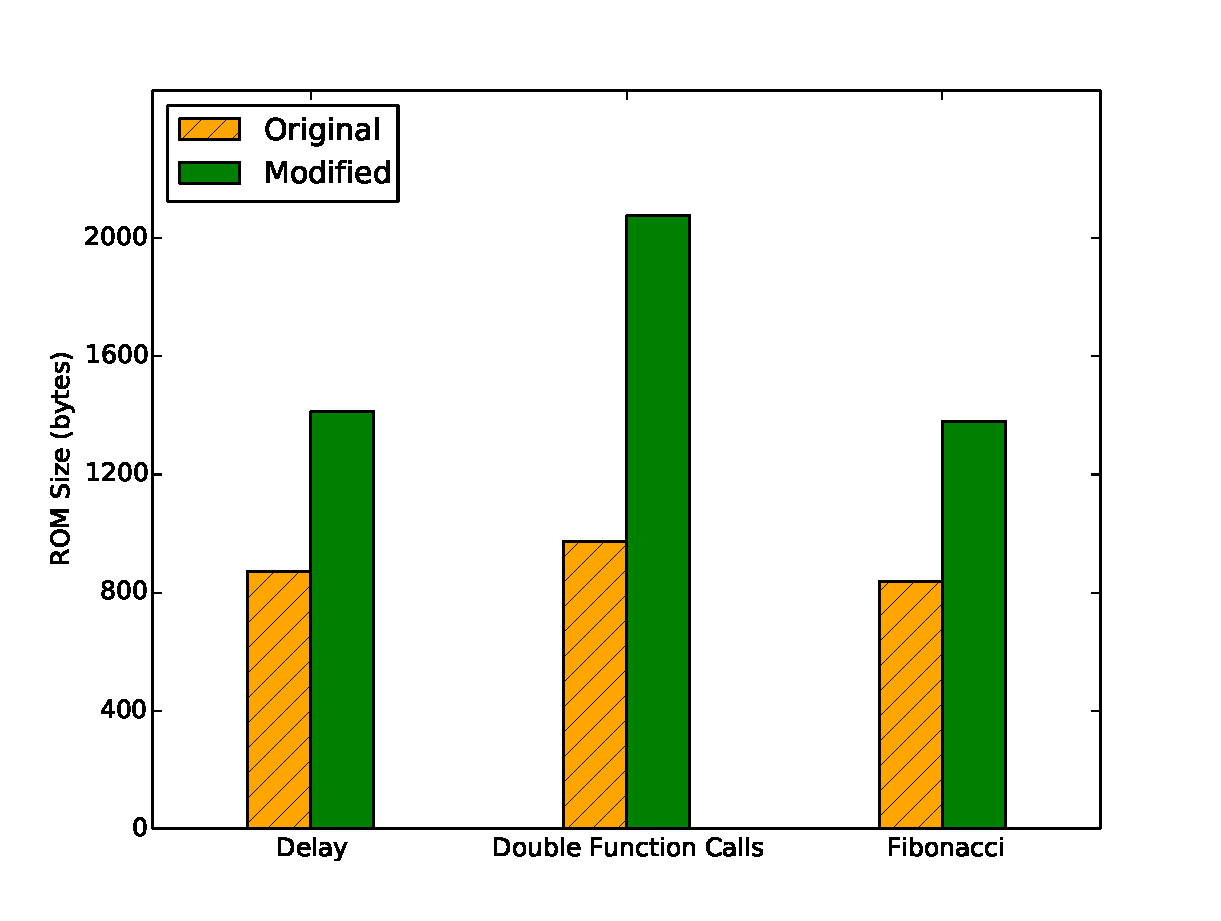
\includegraphics[width=0.3\textwidth]{figures/space_overhead.pdf}
	\end{center}
	\vspace{-15pt}
	\caption{ROM Overhead}
	\vspace{-20pt}
	\label{fig:space_overhead}
\end{wrapfigure}
increasing integer sequence, which is then sent to the UART interface at a controllable speed. A Python program running on a desktop is used to receive the sequence and observe the impact of flipped bits by monitoring the continuity of the sequence. A timer interrupt is used to trigger the occurrence of SEUs. The interrupt service routine generates a random address within the range of the top of the stack and the end of RAM space, excluding the stack frame of the current interrupt, and then flips the bit at this location. 

We declare (observable) failure when one of the following two situations occurs: (i) The AVR application stops generating integers; or (ii) the integer sequence received by the Python program becomes discontinuous. We monitor 
\begin{wrapfigure}{l}{0.50\textwidth}
	\vspace{-30pt}
	\begin{center}
		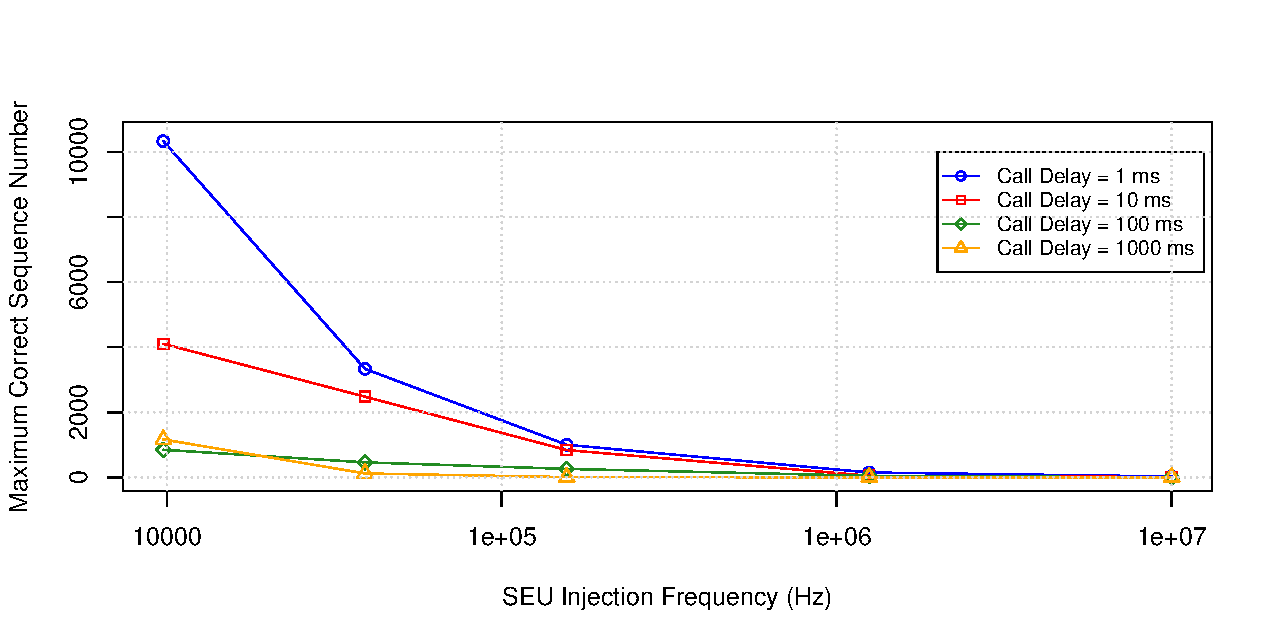
\includegraphics[width=0.50\textwidth]{figures/experiment1.pdf}
	\end{center}
	\vspace{-15pt}
	\caption{Physical Hardware Results}
	\label{fig:exp1_result}
	\vspace{-20pt}
\end{wrapfigure}
the integer sequence and record the maximum count before failure. The experimental results are summarized in Figure \ref{fig:exp1_result}. The x-axis represents SEU injection frequency, and the y-axis represents the maximum count received by the Python program. The figure shows that as SEU injection frequency increases, running time to failure decreases. This is explained as follows: As SEU injection frequency increases, the probability that an SEU occurs in a critical area increases. When the frequency is extremely high (e.g. approximately 10 MHz), the program can hardly send any values. However, the observed SEU occurrence rate in outer space is approximately $10^{-6}SEU/bit$-$Day$~\cite{underwood1992observations}. Given that the total RAM size of an Atmega644 is 4K Bytes, the expected SEU occurrence rate for an Atmega644 is 0.0032 SEU/day, which is significantly lower than the lowest frequency (9765.625 SEU/second) that we used. This situation would be extremely rare in real scenarios.
